\subsection{Vectors}

\content{
}{% presentation
\vspace{3in}
}{% nopresentation
}{% comments
Give a geometric description of vectors. Including scale multiples, and 
the parallelogram rule for adding vectors. Demonstrate vector subtraction
geometrically. Do several examples of combining these operations.
}

\content{
It will be convenient to use vectors along side coordinate systems. If we use
our $x$, $y$, and $z$-axes from before, and we place a vector $\vec{v}$ at the
origin, the terminal end of the vector has coordinates which we will use to
describe the vector itself. 
}{% presentation
\vspace{2in}
}{% nopresentation
}{% comments
Give a few examples of vectors (not necessarily starting at the origin), and
their coordinates.  Introduce $\langle\cdot \rangle $ notation for vectors. 

Give an example of finding a vector between two points in space. 
}

\content{
Each vector has a length associated to it, this can be calculated by the
following formula. 
\begin{definition} The length of a vector $\vec{v} = \langle a_1, a_2\rangle$ is
obtained by the formula 
$$ \sqrt{a_1^2+a_2^2}, $$
and is denoted $|\vec{v}|$. Similarly, for a 3-dimensional vector 
$\vec{u} = \langle a_1, a_2, a_3\rangle$, the length is given by 
$$ |\vec{u}| = \sqrt{a_1^2+a_2^2+a_3^2}. $$
\end{definition}
}{% presentation
}{% nopresentation
}{% comments
}

\content{
When using vectors with a coordinate system, we have a convenient way of
describing the vector operations of addition and scalar multiplication: 
\begin{definition}
If $\vec{v} = \langle a_1,a_2,a_3\rangle$, and $\vec{u} = \langle
b_1,b_2,b_3\rangle$, then 
$$ \vec{v} +\vec{u} = \langle a_1+b_1, a_2+b_2,a_3+b_3\rangle, $$ 
and if $c$ is a scalar, then 
$$ c\vec{v} = \langle ca_1, ca_2,ca_3\rangle. $$
\end{definition}
}{% presentation
}{% nopresentation
}{% comments
}

\content{
\begin{theorem}
if $\vec{a}$, $\vec{b}$, and $\vec{c}$ are vectors, and $c$ and $d$ are scalars,
then the following properties hold: 
\begin{enumerate}
    \item $\vec{a}+ \vec{b} = \vec{b} + \vec{a}$. 
    \item $\vec{a} + (\vec{b}+\vec{c}) = (\vec{a}+\vec{b})+\vec{c}$
    \item $\vec{a} + \vec{0} = \vec{a}$
    \item $\vec{a} + (-\vec{a}) = \vec{0}$
    \item $c(\vec{a}+ \vec{b}) = c\vec{a}+c\vec{b}$
    \item $(c+d)\vec{a} = c\vec{a} + d\vec{a}$
    \item $(cd)\vec{a} = c(d\vec{a})$
    \item $1\vec{a} = \vec{a}$.
\end{enumerate}
\end{theorem}
}{% presentation
}{% nopresentation
}{% comments
}


\content{
\begin{example} If $\vec{a} = \langle 4,0,3\rangle$ and $\vec{b} = \langle
-2,1,5\rangle$, find $a+b$, $a-2b$, $3a$, and $|a|$.
\end{example}
}{% presentation
\vspace{2in}
}{% nopresentation
}{% comments
}


\content{
For 3-dimensional space, there are 3 vectors which play a special role, namely
$$ \vec{i} = \langle 1,0,0\rangle,\quad \vec{j} = \langle 0,1,0\rangle,\quad
\vec{k} = \langle 0,0,1\rangle. $$
These are called the standard basis vectors, and we will often express vectors
in terms of $\vec{i}$, $\vec{j}$, and $\vec{k}$.  For example, we have that 
if $\vec{a} = \langle 3,-2,1\rangle$, then 
$$\vec{a} = \langle 3, -2, 1\rangle  = 3\vec{i} -2\vec{j} + \vec{k}. $$
}{% presentation
}{% nopresentation
}{% comments
}

\content{
\begin{example} For the vectors $\vec{a} = \vec{j} - \vec{k}$ and 
$\vec{b} = 3\vec{i} + 2\vec{j}$, find $\vec{a}+ 2\vec{b}$.
\end{example}
}{% presentation
\vspace{1in}
}{% nopresentation
}{% comments
}

\content{
\begin{definition} A unit vector is a vector whose length is 1.
\end{definition}
The vectors
$\vec{i}$, $\vec{j}$ and $\vec{k}$ are all unit vectors. If we have a vector
$\vec{a}$, and we wish to find a unit vector in the same direction as $\vec{a}$,
we compute 
$$ \vec{u} = \frac{\vec{a}}{|\vec{a}|}. $$
\begin{example} Find a unit vector in the direction of $\langle 2,3,-1\rangle$.
\end{example}
}{% presentation
\vspace{1in}
}{% nopresentation
}{% comments
}

\content{
\begin{example} A 100-lb weight hangs from two wires such that the interior
angles of the wires are $50^\circ$ and $32^\circ$. Find the tension in the two
wires and the magnitudes of these tensions.

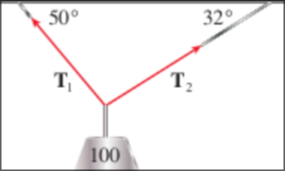
\includegraphics[scale=0.5]{img/load-balance.png}
\end{example}
}{% presentation
}{% nopresentation
}{% comments
The anchor points of the two wires and the point where they support the weight
form a triangle and the top two interior angles are 50 and 32. 

Call the tensions $T_1$ and $T_2$. Then the weight: $-100\vec{j} = T_1 + T_2$.
}
